\documentclass{article}

\usepackage{graphicx}
\usepackage{tikz}
\usepackage{tikzsymbols}
\usetikzlibrary{calc,patterns,shapes.geometric}
\pagestyle{empty}
\usepackage[margin=0pt]{geometry}
\geometry{papersize={14in,12in}}

\def\centerarc[#1](#2)(#3:#4:#5){\draw[#1] ($(#2)+({#5*cos(#3)},{#5*sin(#3)})$) arc (#3:#4:#5);}

\begin{document}
	\begin{figure}
		\centering
		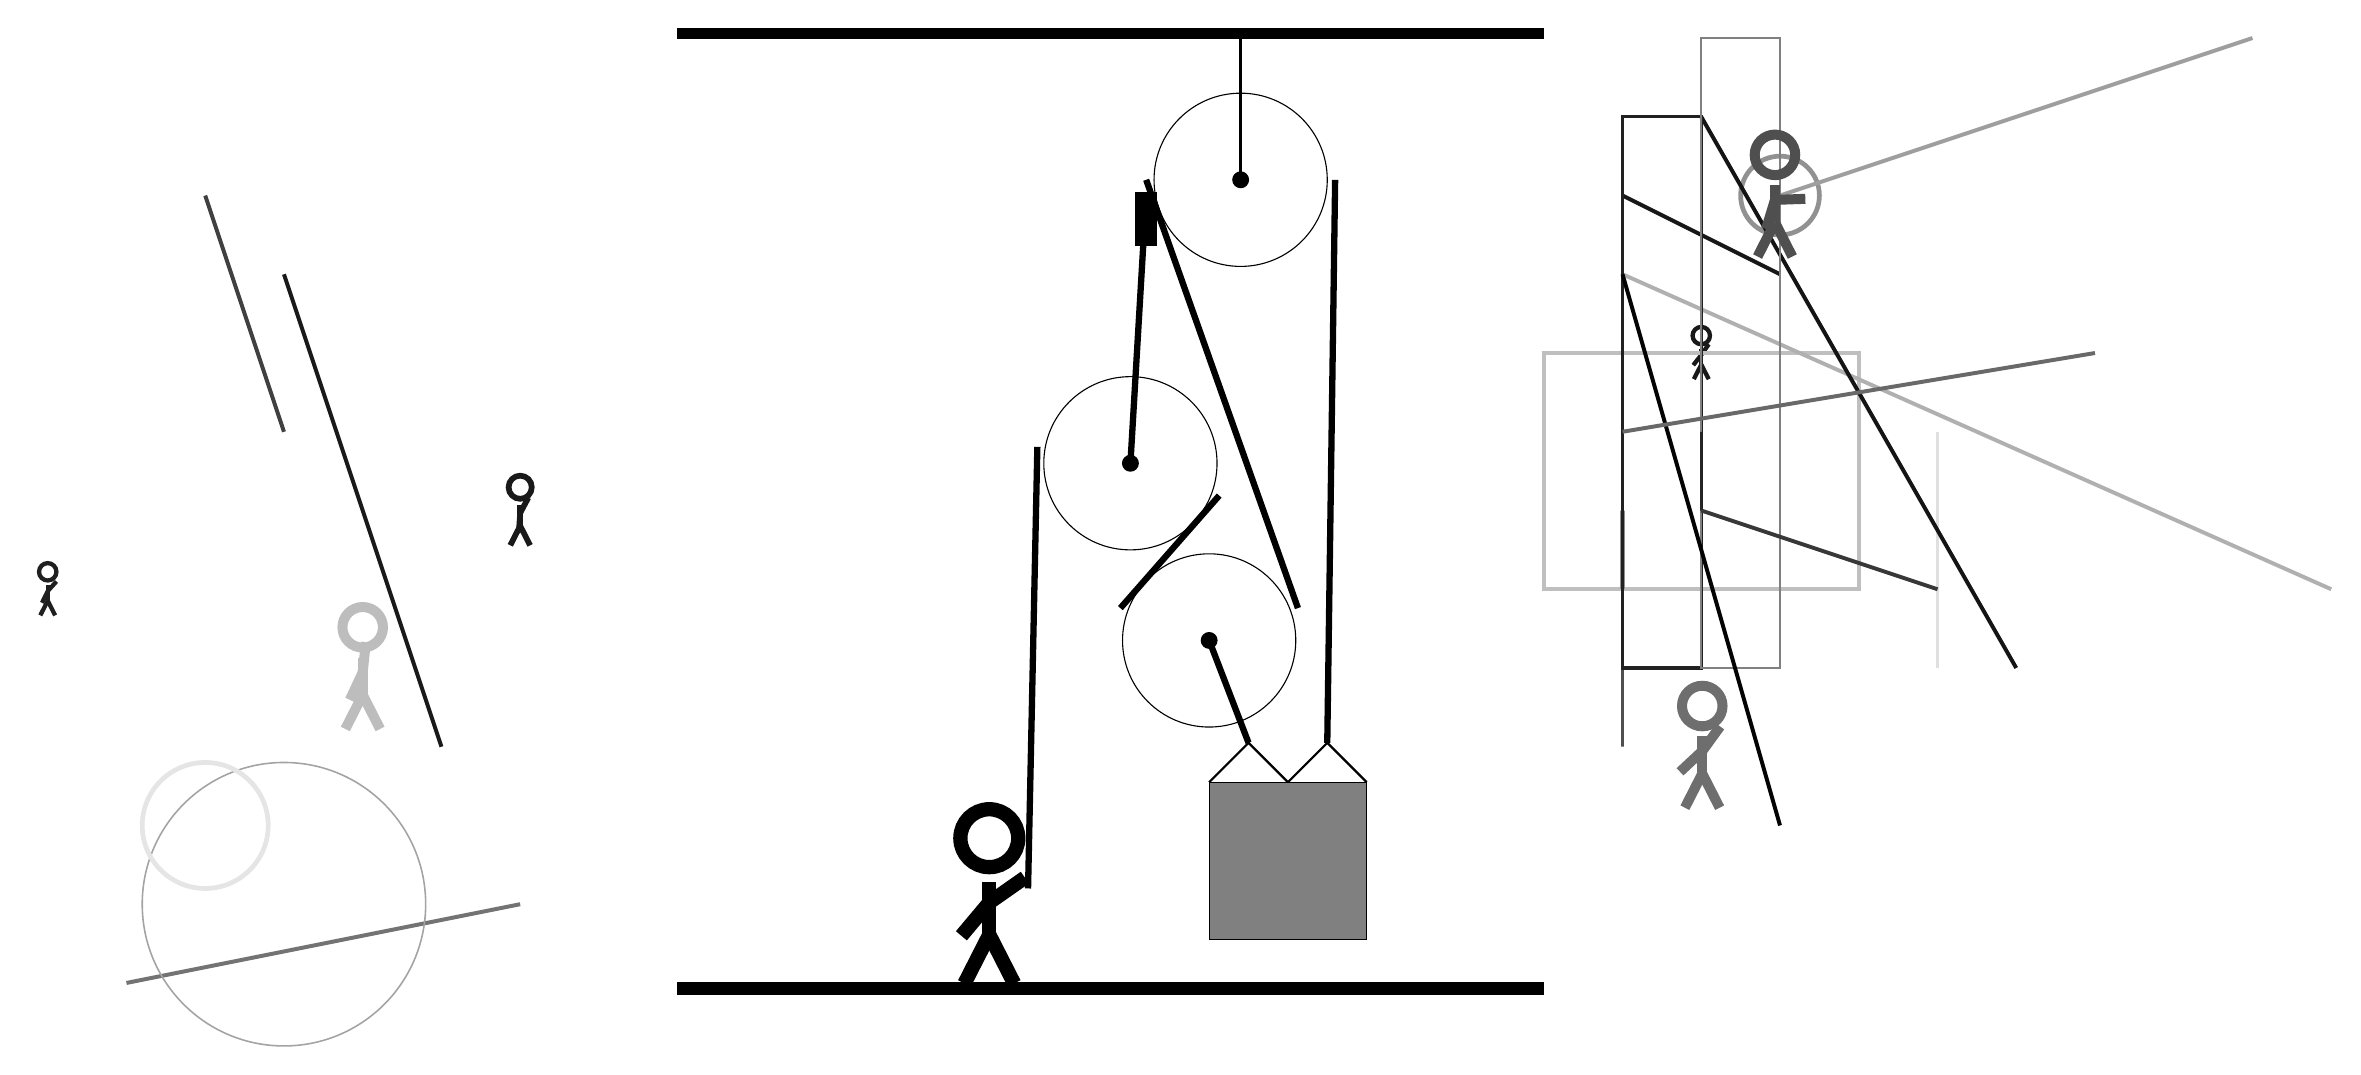
\begin{tikzpicture}
			%%%%% START %%%%%
			
			\draw[fill=black] (-6, 9) rectangle (5, 9.125);
			
			\draw (-0.25, 3.6) circle (1.1);
			\draw[fill=black] (-0.25, 3.6) circle (0.1);
			
			\draw (0.75, 1.35) circle (1.1);
			\draw[fill=black] (0.75, 1.35) circle (0.1);
			
			\draw (1.15, 7.2) circle (1.1);
			\draw[fill=black] (1.15, 7.2) circle (0.1);
			\draw[very thick] (1.15, 7.2) -- (1.15, 9);
			
			\draw[thick]  (0.75, -0.45) -- (1.25, 0.05) -- (1.75, -0.45) -- (2.25, 0.05) -- (2.75, -0.45);
			\draw[fill=black!50] (0.75, -0.45) rectangle (2.75, -2.45);
			
			\draw[line width=0.8mm] (-0.25, 3.6) -- (-0.05, 7.0);
			\draw[line width=0.8mm, fill=black](-0.15, 6.4) rectangle (0.05, 7.0);
			\draw[line width=0.8mm] (-1.55, -1.8) -- (-1.4318, 3.8083);
			\centerarc[line width=0.8mm](-0.25, 3.6)(-20:170:1.2000000000000002);
			\draw[line width=0.8mm] (0.8776, 3.1896) -- (-0.3776, 1.7604);
			\centerarc[line width=0.8mm](0.75, 1.35)(160:380:1.2000000000000002);
			\draw[line width=0.8mm] (1.8776, 1.7604) -- (-0.05, 7.2);
			\draw[line width=0.8mm](0.75, 1.35) -- (1.25, 0.05);
			\centerarc[line width=0.8mm](1.15, 7.2)(0:180:1.2000000000000002);
			\draw[line width=0.8mm] (2.35, 7.2) -- (2.25, 0.05);
			
			\node at (-2, -1.9) {\Strichmaxerl[10][50][35]};
			
			\draw [line width=0.6mm, color=black!43](8, 7) circle (0.5);
			
			\node[line width=0.6mm, color=black!90] at (7, 5) {\Strichmaxerl[3][52][55]};
			\node[line width=0.4mm, color=black!57] at (7, 0) {\Strichmaxerl[7][43][54]};
			\draw[line width=0.5mm, color=black!25] (5, 2) rectangle (9, 5);
			\draw[line width=0.7mm, color=black!43] (6, 2) rectangle (6, 3);
			\node[line width=0.7mm, color=black!88] at (-14, 2) {\Strichmaxerl[3][64][48]};
			
			\draw[line width=0.5mm, color=black!55](-8, -2) -- (-13, -3);
			\draw[line width=0.4mm, color=black!69] (6, 0) rectangle (6, 1);
			\draw[line width=0.5mm, color=black!31](6, 6) -- (15, 2);
			\draw[line width=0.5mm, color=black!12](10, 1) -- (10, 4);
			\draw [line width=0.2mm, color=black!36](-11, -2) circle (1.8);
			\draw[line width=0.5mm, color=black!75](-11, 4) -- (-12, 7);
			\draw[line width=0.5mm, color=black!90](-9, 0) -- (-11, 6);
			
			\draw[line width=0.5mm, color=black!91](8, 6) -- (6, 7);
			\draw[line width=0.5mm, color=black!38](8, 7) -- (14, 9);
			\draw[line width=0.3mm, color=black!85] (7, 5) rectangle (7, 5);
			\draw[line width=0.5mm, color=black!92](7, 8) -- (11, 1);
			\draw[line width=0.4mm, color=black!87] (6, 8) rectangle (7, 1);
			\draw[line width=0.3mm, color=black!50] (7, 1) rectangle (8, 9);
			\node[line width=0.7mm, color=black!26] at (-10, 1) {\Strichmaxerl[7][65][84]};
			\draw[line width=0.5mm, color=black!99](8, -1) -- (6, 6);
			
			\draw[line width=0.3mm, color=black!85] (7, 4) rectangle (7, 3);
			
			\draw [line width=0.6mm, color=black!10](-12, -1) circle (0.8);
			\draw[line width=0.5mm, color=black!59](6, 4) -- (12, 5);
			\node[line width=0.5mm, color=black!69] at (8, 7) {\Strichmaxerl[7][73][2]};
			
			\node[line width=0.5mm, color=black!90] at (-8, 3) {\Strichmaxerl[4][86][62]};
			\draw[line width=0.5mm, color=black!78](7, 3) -- (10, 2);
			
			\draw[fill=black] (-6, -3) rectangle (5, -3.15);
			
			%%%%% END %%%%%
		\end{tikzpicture}
	\end{figure}	
\end{document}